\documentclass[border=6pt]{standalone}
\usepackage{tikz}
\begin{document}
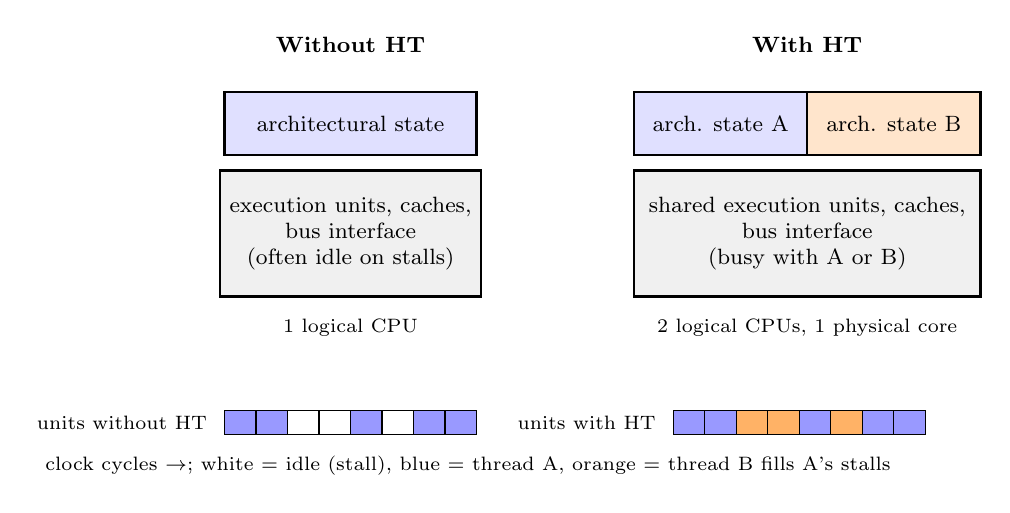
\begin{tikzpicture}[font=\small,
 st/.style={draw,thick,minimum height=0.8cm,align=center,font=\footnotesize},
 ex/.style={draw,thick,minimum height=1.6cm,align=center,font=\footnotesize,fill=gray!12}]
\node[font=\footnotesize\bfseries] at (1.6,2.2) {Without HT};
\node[st,fill=blue!12,minimum width=3.2cm] at (1.6,1.2) {architectural state};
\node[ex,minimum width=3.2cm] at (1.6,-0.2) {execution units, caches,\\bus interface\\(often idle on stalls)};
\node[font=\scriptsize] at (1.6,-1.4) {1 logical CPU};
\begin{scope}[xshift=5.2cm]
\node[font=\footnotesize\bfseries] at (2.2,2.2) {With HT};
\node[st,fill=blue!12,minimum width=2.2cm] at (1.1,1.2) {arch. state A};
\node[st,fill=orange!20,minimum width=2.2cm] at (3.3,1.2) {arch. state B};
\node[ex,minimum width=4.4cm] at (2.2,-0.2) {shared execution units, caches,\\bus interface\\(busy with A or B)};
\node[font=\scriptsize] at (2.2,-1.4) {2 logical CPUs, 1 physical core};
\end{scope}
% thread activity strip
\begin{scope}[yshift=-2.6cm]
\node[font=\scriptsize,anchor=east] at (-0.1,0) {units without HT};
\foreach \x/\c in {0/blue!40,1/blue!40,2/white,3/white,4/blue!40,5/white,6/blue!40,7/blue!40} \draw[fill=\c] (\x*0.4,-0.15) rectangle (\x*0.4+0.4,0.15);
\node[font=\scriptsize,anchor=east] at (5.6,0) {units with HT};
\foreach \x/\c in {0/blue!40,1/blue!40,2/orange!60,3/orange!60,4/blue!40,5/orange!60,6/blue!40,7/blue!40} \draw[fill=\c] (5.7+\x*0.4,-0.15) rectangle (5.7+\x*0.4+0.4,0.15);
\node[font=\scriptsize,anchor=north west] at (-2.4,-0.3) {clock cycles $\to$; white = idle (stall), blue = thread A, orange = thread B fills A's stalls};
\end{scope}
\end{tikzpicture}
\end{document}
